\documentclass[11pt]{article}

\usepackage[T1]{fontenc}
\usepackage[utf8]{inputenc}
\usepackage{lmodern}
\usepackage{microtype}
\usepackage{amsmath}
\usepackage[margin=1in]{geometry}
\usepackage{setspace}
\usepackage{graphicx}
\usepackage{booktabs}
\usepackage{tabularx}
\usepackage{longtable}
\usepackage{xurl}
\usepackage{etoolbox}

\usepackage{array}
\usepackage{adjustbox}
\usepackage{float}
\usepackage[font=small,labelfont=bf]{caption}
\usepackage{xcolor}
\usepackage{hyperref}
\usepackage{fancyhdr}
\usepackage{enumitem}
\usepackage[numbers,sort&compress]{natbib}

\graphicspath{{figs/}}
\definecolor{accent}{HTML}{1F4E79}
\hypersetup{
  colorlinks=true,
  linkcolor=accent,
  citecolor=accent,
  urlcolor=accent,
  pdftitle={Tree Model Comparison on the UCI Mushroom Dataset},
  pdfauthor={Uzayr Chaudhry and David Mwaria}
}
\setlength{\parindent}{0pt}
\setlength{\parskip}{0.35em}
\setlength{\tabcolsep}{5pt}
\renewcommand{\arraystretch}{1.12}
\setlist[itemize]{leftmargin=1.5em,itemsep=0.2em,topsep=0.3em}

\pagestyle{fancy}
\setlength{\headheight}{14pt}
\fancyhf{}
\fancyhead[L]{CS 4372: Tree Model Comparison}
\fancyhead[R]{Chaudhry and Mwaria}
\fancyfoot[C]{\thepage}
\renewcommand{\headrulewidth}{0.4pt}

\begin{document}

\pagenumbering{roman}
\begin{titlepage}
  \thispagestyle{empty}
  \centering
  \vspace*{1.15in}

  {\Large\textcolor{accent}{CS 4372}\par}
  \vspace{0.35in}
  {\Huge\bfseries Tree Model Comparison on the UCI Mushroom Dataset\par}
  \vspace{0.25in}
  {\Large Classifying edible and poisonous mushrooms\par}

  \vspace{0.55in}
  \rule{0.78\textwidth}{0.6pt}
  \vspace{0.5in}

  {\large
  \begin{tabular}{>{\bfseries}rl}
    Team member: & Uzayr Chaudhry \\
    NetID: & uxc230006 \\
    \addlinespace[0.3em]
    Team member: & David Mwaria \\
    NetID: & dmm240001 \\
  \end{tabular}
  \par}

  \vfill
  {\large The University of Texas at Dallas\par}
  \vspace{0.12in}
  {\large Instructor: A. Nagar\par}
  \vspace{0.4in}
  {\small Dataset: UCI Machine Learning Repository, Mushroom\par}
  {\small\url{https://archive.ics.uci.edu/dataset/73/mushroom}\par}
\end{titlepage}

\pagenumbering{arabic}

\begin{abstract}
Four tree methods achieve perfect classification and ranking on the Mushroom test set. The central result is not an ensemble advantage: a small set of categorical rules already separates these labels. We test conditional feature removal, trace rare Decision Tree paths, and distinguish probability quality from classification. Every test row repeats a training combination of the five selected traits. A stress test holds groups defined by those traits apart, while refitting feature selection within each fold. All four methods then miss the same three positive odorless profiles. XGBoost reduces false positives, but does not recover these exceptions. The main finding is that strong aggregate scores can conceal complete failure on a small subgroup.
\end{abstract}

\section{What is being predicted?}
Each row describes mushroom morphology, odor and habitat. The cap is the mushroom top, the gills are underneath it, and the stalk is the stem. Ring traits describe a band around the stalk; spore print color is the color of deposited spores. Above-ring and below-ring traits describe different stem sections. The 22 predictors are recorded categories. Most are nominal; ring count and gill width have ordered meanings. We use a common one-hot representation for all of them. We predict the edible label versus the UCI poisonous label, with poisonous treated as positive. UCI groups unknown edibility with the poisonous category. Thus the target is a source-defined label, not a measured probability of human poisoning. The 8,124 descriptions cover hypothetical samples from 23 species; no species identifier is available for evaluation \cite{ucimushroom}.

The data contain 4,208 edible and 3,916 positive records. Neither class is rare. F1 balances positive-class precision and recall and is the scoring objective used throughout the reported grid searches. It does not encode a known cost of false negatives. In particular, our default decision threshold does not establish a safety policy. The public UCI source is accessed through its Python client; no raw dataset is submitted.

\section{Audit and representation}
\begin{table}[H]
\centering\small
\caption{Audit of the original Mushroom records.}
\begin{tabular}{lr}
\toprule
Check & Count \\
\midrule
Rows & 8124 \\
Predictors & 22 \\
Missing cells & 2480 \\
Duplicate rows & 0 \\
Duplicate predictor rows & 0 \\
Edible & 4208 \\
Poisonous / not recommended & 3916 \\
\bottomrule
\end{tabular}
\end{table}

All observed category codes match the source dictionary. There are no exact duplicate predictor rows or complete rows. These checks establish internal consistency, not independent specimen sampling. The sole missing attribute is stalk root: 2,480 entries, or 30.53\%. We preserve these rows and represent missing root as an explicit unknown category inside each fitted pipeline. Imputation with a frequent root would invent anatomy. The source API calls cap color binary, but ten observed levels establish that it must be treated as nominal. Veil type is constant (partial veil) and is removed within each training fold. Ring type ``none'' and ring number ``none'' agree in every record.

Missingness is informative in this sample: among training rows, 1,402 of 1,990 missing-root records are positive (70.45\%), compared with 38.39\% when root is known. That association does not identify why values are missing or prove that missingness causes the label. The selected models exclude stalk root, so their predictions do not rely on this indicator.

We summarize all attributes using category frequencies and provide class-conditional counts for odor and the selected traits, with a full dictionary in the notebook exports. Normality is not meaningful for unordered letter codes. Ring count is also a discrete category with only three possible values, rather than a Gaussian quantity. A normality test on arbitrary integers would measure the coding scheme rather than morphology. One-hot encoding avoids imposing distances or an order. After constant removal, the full training representation has 116 indicator columns. Rare levels are retained, including four conical caps and four grooved cap surfaces in training; their small support limits interpretation. The appendix shows selected-trait counts; the full distribution plot and all frequencies are supplied with the notebook.

We demonstrate both training-fitted standardization and min-max normalization. The notebook exports training and test summaries in scaling\_summary.csv, including ranges, column means and column standard deviations. Standardization centers each indicator and rescales it by its training standard deviation. Min-max scaling maps its training range to $[0,1]$. These are separate demonstrations, not successive transformations. The model pipeline uses min-max scaling after encoding; nonconstant binary indicators already span $[0,1]$, so this transformation changes neither their values nor tree split ordering. Scaling satisfies the preprocessing requirement but supplies no predictive advantage here. Unknown future category levels are ignored by the encoder, a computational fallback whose accuracy is not established by this dataset.

\section{What explains the labels?}
A profile is an exact combination of recorded traits, such as odorless, green-spored, broad-gilled mushrooms with a pendant ring and smooth lower stalk. A feature policy specifies which traits the model may retain; a ranked prefix consists of the first traits in their training association ranking. We measure categorical association with Cramer's $V$, computed from contingency tables. It is zero for independence and can reach one for strong association; constant predictors are excluded. Unlike Pearson correlation of letter codes, this statistic is invariant to category renaming. The numerical matrices and training-only heatmaps provide both predictor-to-target and predictor-to-predictor evidence. These uncorrected descriptive values are not causal effects or significance tests; unequal category support and rare levels matter.

\begin{figure}[H]\centering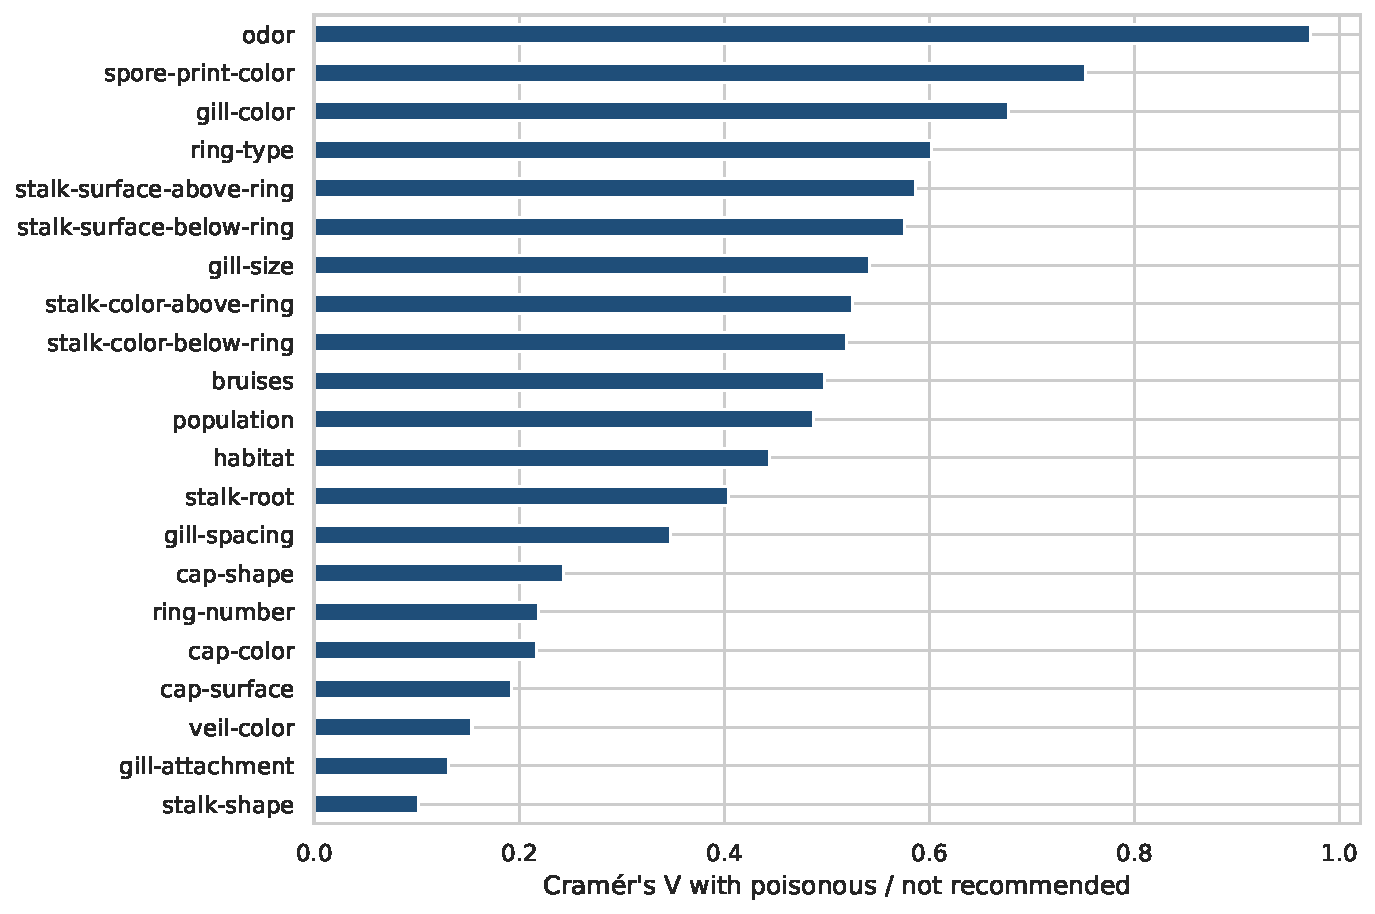
\includegraphics[width=.88\linewidth]{03_target_associations.pdf}\caption{Training associations with the positive label. Marginal strength is not conditional usefulness.}\end{figure}
Odor has the strongest marginal association ($V=0.9716$). Spore print color follows ($0.7526$), then gill color ($0.6776$). These figures motivate a ranking, but a high rank need not imply incremental value. Gill color disappears from the smaller successful policy once the other traits are known. This is why removal tests are more informative than merely repeating the ranking.

\begin{figure}[H]\centering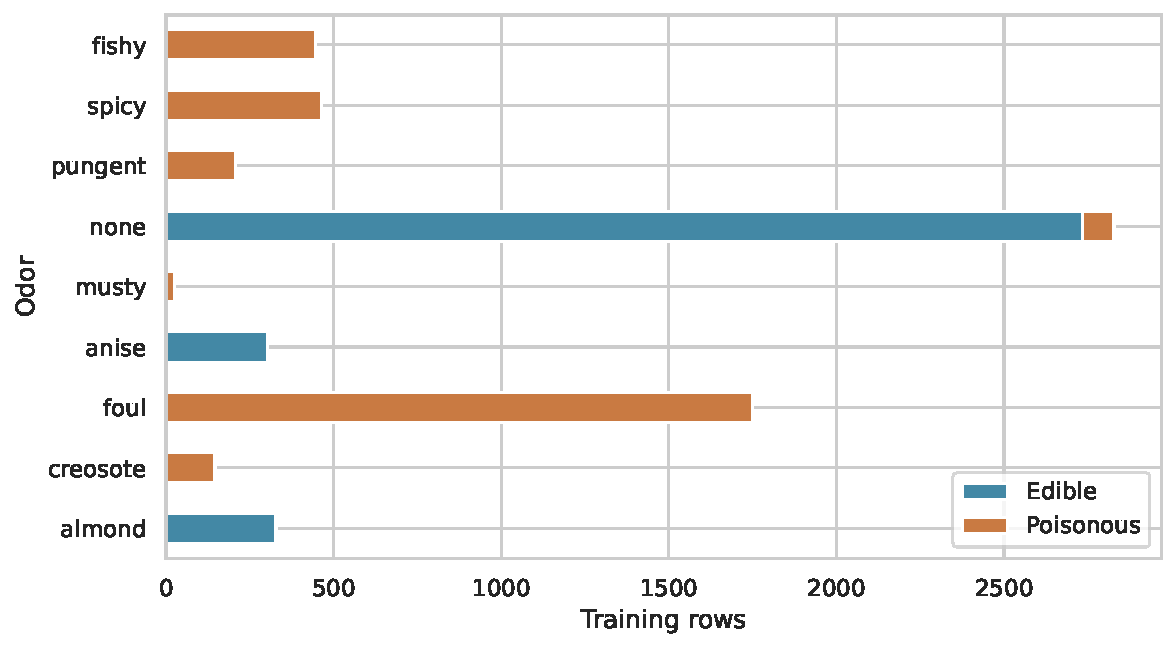
\includegraphics[width=.9\linewidth]{15_odor_class_counts.pdf}\caption{Training odor counts by class. Odorless records contain the important minority of positive exceptions.}\end{figure}
Odor is a strong first approximation rather than a complete explanation. A training-learned odor-category majority rule classifies almond, anise and odorless rows as edible and other observed odors as positive. It misses 26 of the 783 positive test records, all odorless, while producing no false positives. Its F1 is 0.9831. The remaining traits matter because they resolve this small exceptional subgroup, not because they improve every prediction equally.
\begin{table}[H]
\centering\small
\caption{Predefined test-set baselines. Poisonous is positive.}
\begin{adjustbox}{max width=\linewidth}\begin{tabular}{lrrrrrr}
\toprule
Baseline & Accuracy & Precision & Recall & F1 & FN & FP \\
\midrule
Always edible & 0.5182 & 0.0000 & 0.0000 & 0.0000 & 783 & 0 \\
Always poisonous & 0.4818 & 0.4818 & 1.0000 & 0.6503 & 0 & 842 \\
Odor category majority & 0.9840 & 1.0000 & 0.9668 & 0.9831 & 26 & 0 \\
\bottomrule
\end{tabular}\end{adjustbox}
\end{table}


The largest pairwise associations involve gill attachment and stalk colors ($V=0.9815$) and attachment with veil color ($0.9593$). These large values partly reflect constrained, uneven category combinations. They do not make the traits interchangeable for every prediction. Upper and lower stalk colors have $V=0.6420$; the two stalk surfaces have $V=0.4950$. Consequently, a pairwise cutoff of 0.90 cannot detect all conditional redundancy. We compare that screen with unscreened policies and use validation to decide. Correlated traits can affect feature sampling in a forest and distribute importance across alternatives; trees do not require the absence of correlation.

\section{Validation and deliberate feature selection}
The original stratified split contains 6,499 training and 1,625 test rows, with seed 4372. Five shuffled stratified folds, also seeded 4372, are used for GridSearchCV. Selection, unknown-category handling, encoding and scaling are fitted inside each fold. Training labels drive feature ranking; validation labels score it. The test partition is excluded from fitting and grid scoring. The reduced policies cap the retained prefix at its size minus the number of named exclusions, so changed rankings cannot exceed the declared trait limit. The same test set was evaluated in earlier project versions and is retained for comparison. Final feature policies and hyperparameters are selected using training cross-validation. The test results are not presented as a newly blind confirmation.

Each model searches ranked prefixes of 6, 7, 8, 9, 10 and 21 traits, with and without the pairwise screen. Earlier training diagnostics found that gill color and upper stalk surface could be jointly removed from the seven-trait policy. We add that five-trait candidate and each of its five single-trait removals. This is a targeted comparison, not exhaustive search over all subsets. Fold-local ranking can change which traits enter a prefix; the exported fold diagnostics retain those choices.

Exact F1 ties use a declared preference: fewer permitted traits, no pairwise screen, shallower trees, fewer estimators, larger minimum leaves, then lower learning rate. This resolves ties within the grid; it does not establish a unique global optimum or minimum tree size. We retain all fold scores and training scores in the four grid CSV files, including configurations that fail to reach the ceiling.
\begin{table}[H]
\centering\small
\caption{Selected cross-validation results.}
\begin{tabular}{lrrrr}
\toprule
Model & Candidates & CV F1 & CV SD & Attributes \\
\midrule
Decision Tree & 108 & 1.0000 & 0.0000 & 5 \\
Random Forest & 288 & 1.0000 & 0.0000 & 5 \\
AdaBoost & 216 & 1.0000 & 0.0000 & 5 \\
XGBoost & 144 & 1.0000 & 0.0000 & 5 \\
\bottomrule
\end{tabular}
\end{table}

\textbf{Attributes selected by all four final models:} odor, spore-print-color, ring-type, stalk-surface-below-ring, gill-size.

\textbf{Decision Tree}: max\_depth=6; min\_samples\_leaf=5\\
\textbf{Random Forest}: max\_depth=6; max\_features=0.7; min\_samples\_leaf=3; n\_estimators=100\\
\textbf{AdaBoost}: base\_max\_depth=1; learning\_rate=1.0; n\_estimators=150\\
\textbf{XGBoost}: learning\_rate=0.2; max\_depth=2; n\_estimators=250

The grid tests depth and leaf regularization for the Decision Tree; tree count, depth, leaf size and encoded-feature sampling for the forest; weak-tree depth, learning rate and estimator count for AdaBoost; and depth, learning rate and boosting rounds for XGBoost. These implementations follow the course model families \cite{nagarnotebooks,sklearnensembles,xgbintro}. These parameters control distinct mechanisms: a shallow tree may omit an exceptional path, while boosting with small updates may need more rounds to resolve it. A forest can miss a dominant trait when sampling too few indicator columns. Feature sampling is applied to encoded columns, not the original trait count.

The strongest searched configurations hit mean F1 1.0 in row validation. At that ceiling, increasing the grid cannot demonstrate an F1 improvement. We therefore justify the chosen values by the searched alternatives and the tie preference, not a claim that all possible parameter values were explored. The selected-policy grid tables retain the evidence needed to compare each setting. The following table isolates variation in model settings while holding the chosen feature policy fixed.
\begin{table}[H]
\centering\small
\caption{Sensitivity to model settings within each selected feature policy.}
\begin{adjustbox}{max width=\linewidth}\begin{tabular}{lrrrr}
\toprule
Model & Best F1 & Worst F1 & Settings & Perfect F1 settings \\
\midrule
Decision Tree & 1.0000 & 0.9963 & 6 & 4 \\
Random Forest & 1.0000 & 0.9928 & 16 & 12 \\
AdaBoost & 1.0000 & 0.9690 & 12 & 4 \\
XGBoost & 1.0000 & 0.9939 & 8 & 4 \\
\bottomrule
\end{tabular}\end{adjustbox}
\end{table}
 Within the five-trait policy, depth-three Decision Trees reach F1 0.9963; depth six reaches 1.0 and unlimited depth adds no benefit. The forest has 29 indicator columns. At depth six, square-root feature sampling considers five columns and reaches at most 0.9939; sampling 70 percent considers 20 and reaches 1.0. Additional trees cannot recover that gap as effectively within this grid. AdaBoost with stumps and rate 0.1 reaches only 0.9748 at 150 rounds; rate 1.0 reaches 1.0. XGBoost at depth two and rate 0.2 moves from 0.9987 at 100 rounds to 1.0 at 250. These comparisons establish sensitivity to model settings and are consistent with difficulty resolving rare exceptions. They do not identify which validation cases change under each setting. Larger settings beyond the ceiling give no observed F1 gain.
Reported CV standard deviations are variation among the five folds, not confidence intervals after model selection.

With the selected Decision Tree settings fixed, removing odor gives F1 0.9798; removing spore-print-color gives F1 0.9897; removing ring-type gives F1 0.9987; removing stalk-surface-below-ring gives F1 0.9944; removing gill-size gives F1 0.9987. This tests conditional contribution within that fitted policy. It neither proves that a trait is inherently necessary nor rules out replacement by another untested trait.
\begin{table}[H]
\centering\small
\caption{Removal from the selected Decision Tree policy, with model settings fixed.}
\begin{tabular}{lrr}
\toprule
Removed attribute & CV F1 & CV SD \\
\midrule
None & 1.0000 & 0.0000 \\
odor & 0.9798 & 0.0030 \\
spore-print-color & 0.9897 & 0.0022 \\
ring-type & 0.9987 & 0.0010 \\
stalk-surface-below-ring & 0.9944 & 0.0017 \\
gill-size & 0.9987 & 0.0010 \\
\bottomrule
\end{tabular}
\end{table}

\begin{table}[H]
\centering\small
\caption{Training profiles with contradictory labels after removal from the selected policy.}
\begin{adjustbox}{max width=\linewidth}\begin{tabular}{lrrrrr}
\toprule
Removed & Attributes & Profiles & Mixed-label profiles & Mixed rows & Min. training errors \\
\midrule
None & 5 & 47 & 0 & 0 & 0 \\
odor & 4 & 29 & 3 & 1181 & 129 \\
spore-print-color & 4 & 28 & 2 & 1817 & 64 \\
ring-type & 4 & 43 & 1 & 24 & 8 \\
stalk-surface-below-ring & 4 & 33 & 1 & 62 & 30 \\
gill-size & 4 & 41 & 1 & 153 & 8 \\
\bottomrule
\end{tabular}\end{adjustbox}
\end{table}

Removing each selected trait also creates mixed-label training profiles in the remaining representation. Within these particular subsets, an identical input then requires two different labels, so no deterministic classifier on those inputs can reproduce both. The minimum training-error column sums the minority class count in each profile, giving a representation-specific error floor. This is a training consistency bound, not a bound on future error. This gives a structural reason for the loss rather than merely reporting a lower score. It establishes irreducibility relative to the tested five-trait representation, not a global minimum across all 22 traits.

\section{What the fitted trees actually do}
\begin{table}[H]
\centering\small
\caption{Complexity of the fitted models.}
\begin{adjustbox}{max width=\linewidth}\begin{tabular}{lrrr}
\toprule
Model & Trees & Max fitted depth & Total leaves \\
\midrule
Decision Tree & 1 & 6 & 10 \\
Random Forest & 100 & 6 & 1106 \\
AdaBoost & 150 & 1 & 300 \\
XGBoost & 250 & 2 & 836 \\
\bottomrule
\end{tabular}\end{adjustbox}
\end{table}

The Decision Tree exposes the rule sequence directly. Each decoded split tests a one-hot indicator; a threshold at 0.5 distinguishes category absence from presence. Odor distinguishes common cases; spore print, lower stalk surface, gill size and ring type resolve odorless exceptions when those traits are present in its chosen representation. The complete decoded path file records the exact conjunctions rather than treating any one category as a universal rule. Leaves separate the training labels, but their support varies sharply. The table below identifies paths with little or no test evidence.
\begin{table}[H]
\centering\small
\caption{Decision Tree leaf support. Complete conditions are exported in decision\_paths.csv.}
\begin{adjustbox}{max width=\linewidth}\begin{tabular}{rlrrrr}
\toprule
Leaf & Prediction & Train rows & Train poisonous & Test rows & Test poisonous \\
\midrule
3 & poisonous & 3039 & 3039 & 757 & 757 \\
4 & edible & 304 & 0 & 96 & 0 \\
5 & edible & 328 & 0 & 72 & 0 \\
9 & edible & 2573 & 0 & 627 & 0 \\
11 & edible & 114 & 0 & 30 & 0 \\
13 & poisonous & 8 & 8 & 0 & 0 \\
14 & edible & 32 & 0 & 16 & 0 \\
16 & poisonous & 30 & 30 & 10 & 10 \\
17 & edible & 15 & 0 & 1 & 0 \\
18 & poisonous & 56 & 56 & 16 & 16 \\
\bottomrule
\end{tabular}\end{adjustbox}
\end{table}

The smallest positive leaf uses this conjunction: odor = none; not (spore-print-color = green); not (stalk-surface-below-ring = scaly); gill-size = narrow; spore-print-color = white; not (ring-type = evanescent). It contains 8 training rows, all positive, and 0 test rows. That support explains why aggregate perfection gives limited evidence for this particular exception.
A leaf with zero test rows has not been independently checked by that partition. A pure leaf supported by only a few descriptions should not be interpreted as a biological certainty. The complete Decision Tree is exported separately so its deepest paths remain readable.

\begin{figure}[H]\centering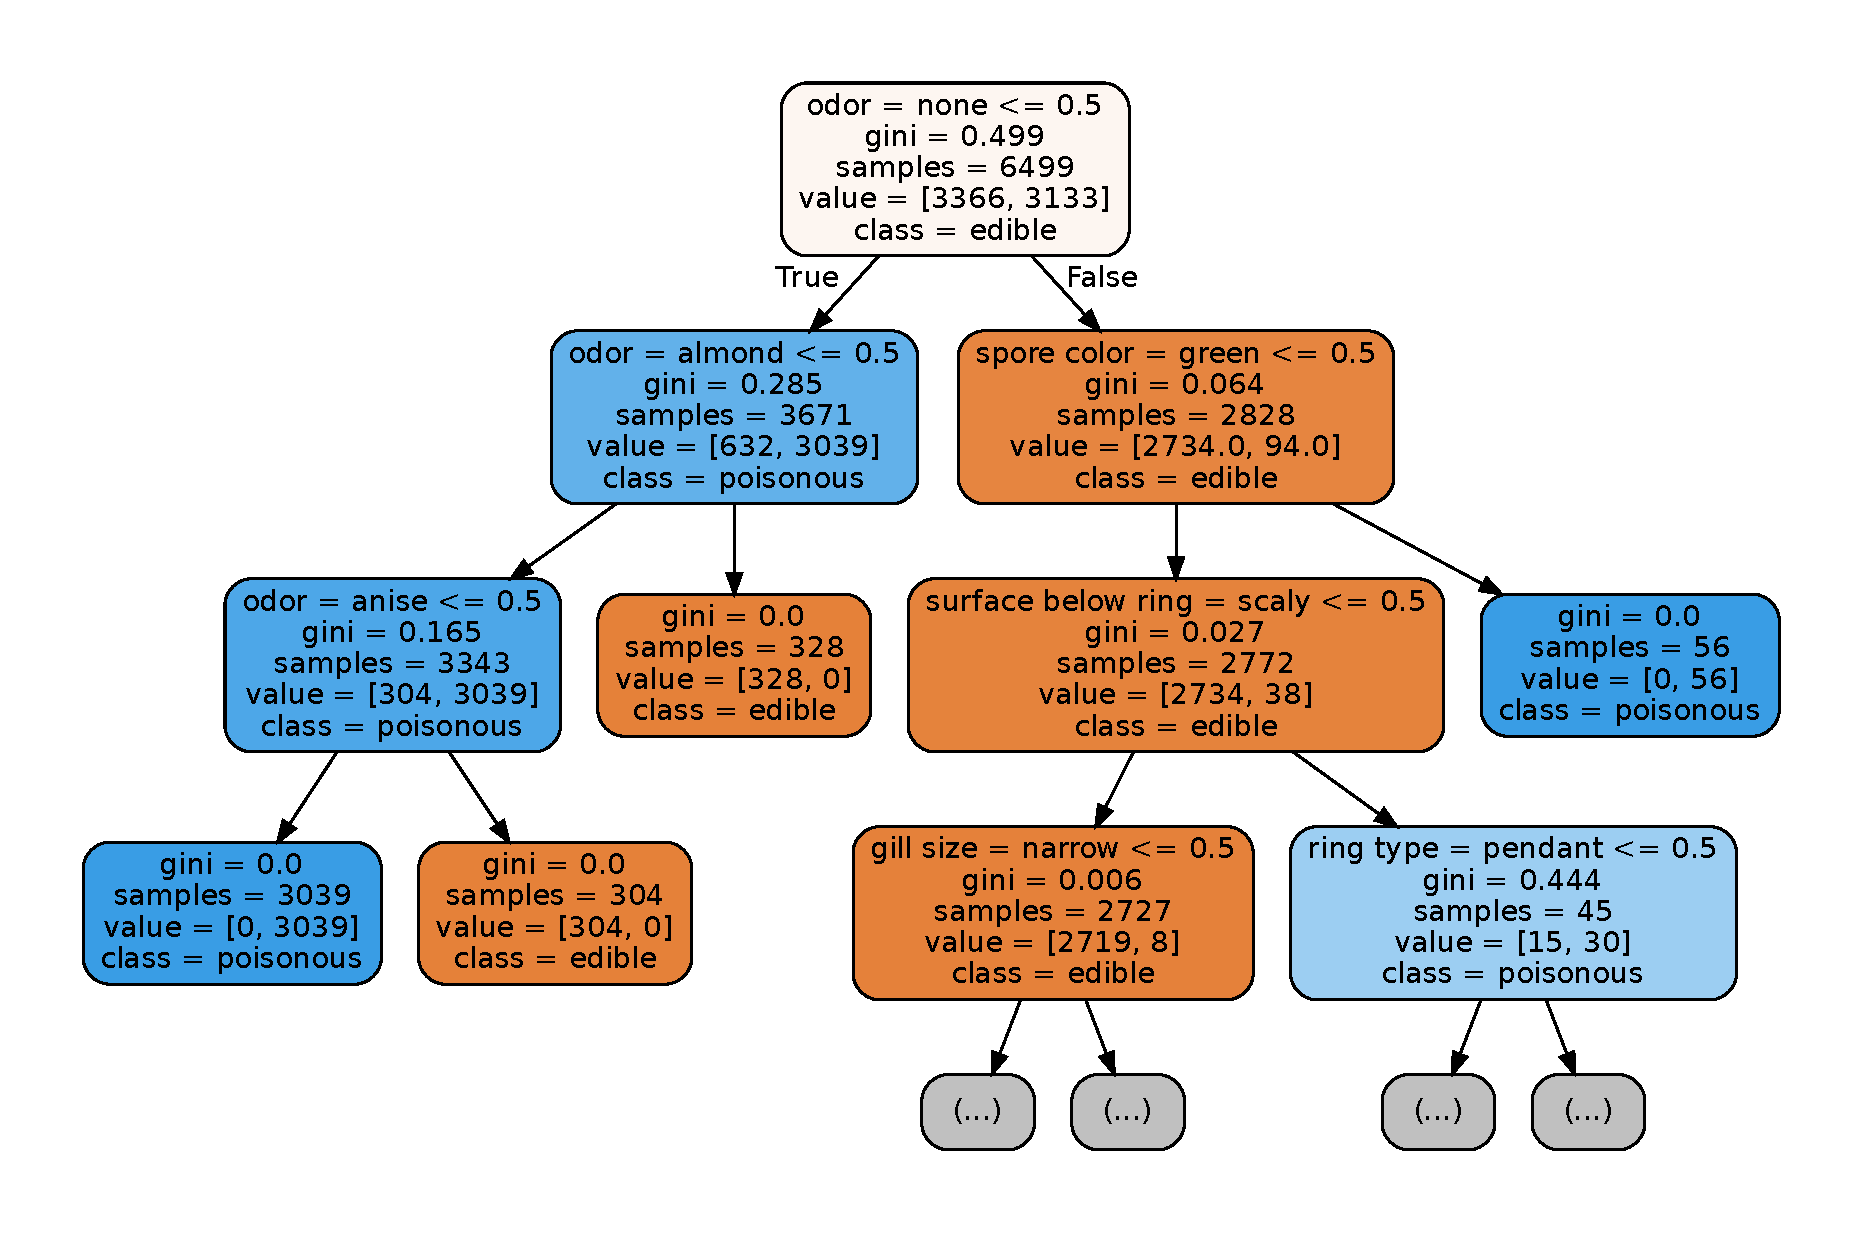
\includegraphics[width=.9\linewidth]{05_decision_tree.pdf}\caption{Root and first three split depths of the fitted Decision Tree. Ellipses hide deeper decisions; the full tree is supplied in figs/.}\end{figure}
The forest combines trees fitted to bootstrap samples and random encoded-feature subsets. Its displayed first tree is an illustration, not the forest's entire decision rule. The displayed sample counts refer to distinct contributing rows within that bootstrap draw; repeated rows contribute through weights. AdaBoost combines weak trees and emphasizes observations misclassified at earlier rounds. Its first tree cannot alone represent the full classifier. XGBoost adds successive tree contributions to a score transformed into a probability; the displayed leaf numbers are contributions to log odds, not class probabilities. The ensemble plots in the appendix make these distinctions explicit. Their greater fitted complexity does not automatically yield better test-set predictions.

\section{Classification, ranking and probability are different claims}
The test contains 842 edible and 783 positive records. A false negative is a positive record predicted edible; a false positive reverses that assignment. Precision is $TP/(TP+FP)$, recall is $TP/(TP+FN)$, and F1 is their harmonic mean. We use F1 in place of the assignment's ``F-statistic.''
\begin{table}[H]
\centering\small
\caption{Classification and ranking on the previously evaluated test set.}
\begin{adjustbox}{max width=\linewidth}\begin{tabular}{lrrrrrr}
\toprule
Model & Accuracy & Precision & Recall & F1 & ROC AUC & Average precision \\
\midrule
Decision Tree & 1.0000 & 1.0000 & 1.0000 & 1.0000 & 1.0000 & 1.0000 \\
Random Forest & 1.0000 & 1.0000 & 1.0000 & 1.0000 & 1.0000 & 1.0000 \\
AdaBoost & 1.0000 & 1.0000 & 1.0000 & 1.0000 & 1.0000 & 1.0000 \\
XGBoost & 1.0000 & 1.0000 & 1.0000 & 1.0000 & 1.0000 & 1.0000 \\
Majority baseline & 0.5182 & 0.0000 & 0.0000 & 0.0000 & 0.5000 & 0.4818 \\
\bottomrule
\end{tabular}\end{adjustbox}
\end{table}

\begin{figure}[H]\centering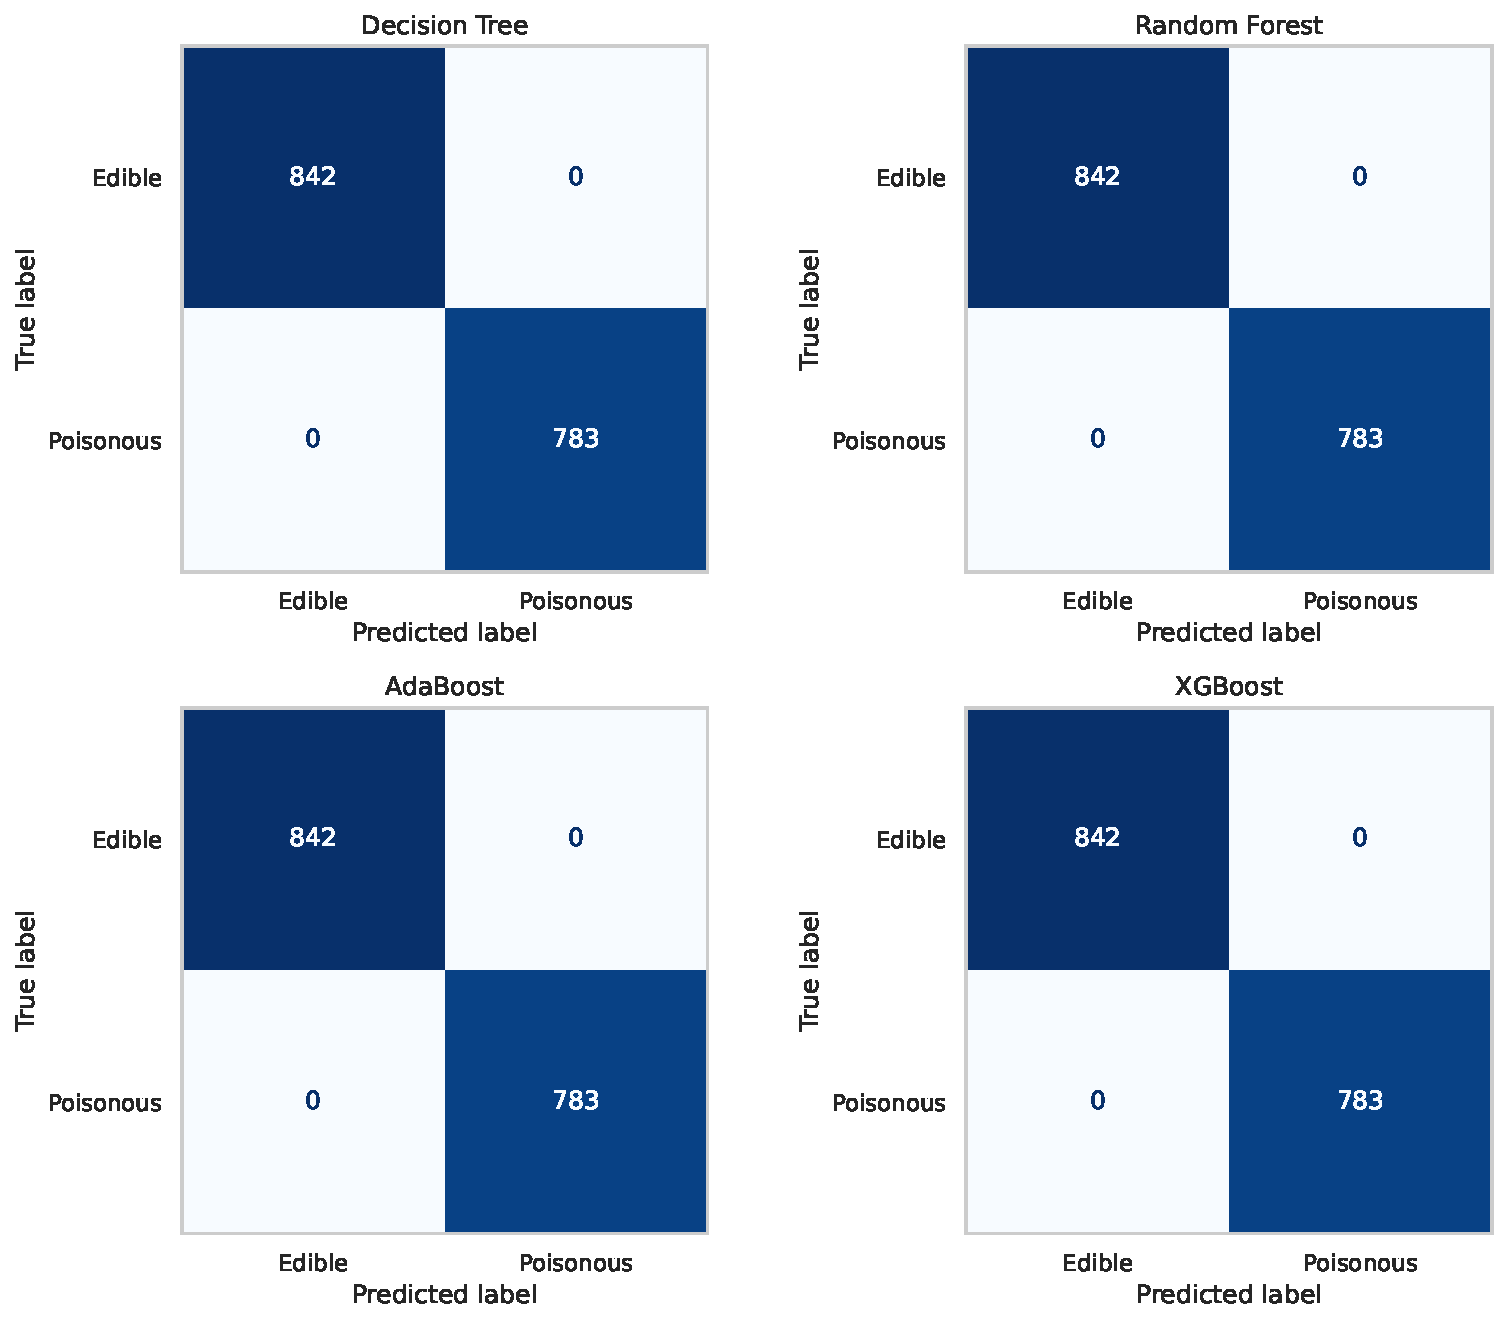
\includegraphics[width=.85\linewidth]{09_confusion_matrices.pdf}\caption{Default operating-point decisions on the previously evaluated test set. The class counts make error totals auditable.}\end{figure}
All four methods place all test labels correctly at their default threshold. The confusion matrices establish zero observed false negatives and false positives here; they do not establish zero future risk. Accuracy alone would conceal the odor-only rule's positive-class misses, which is why its recall and F1 also matter.

\begin{figure}[H]\centering
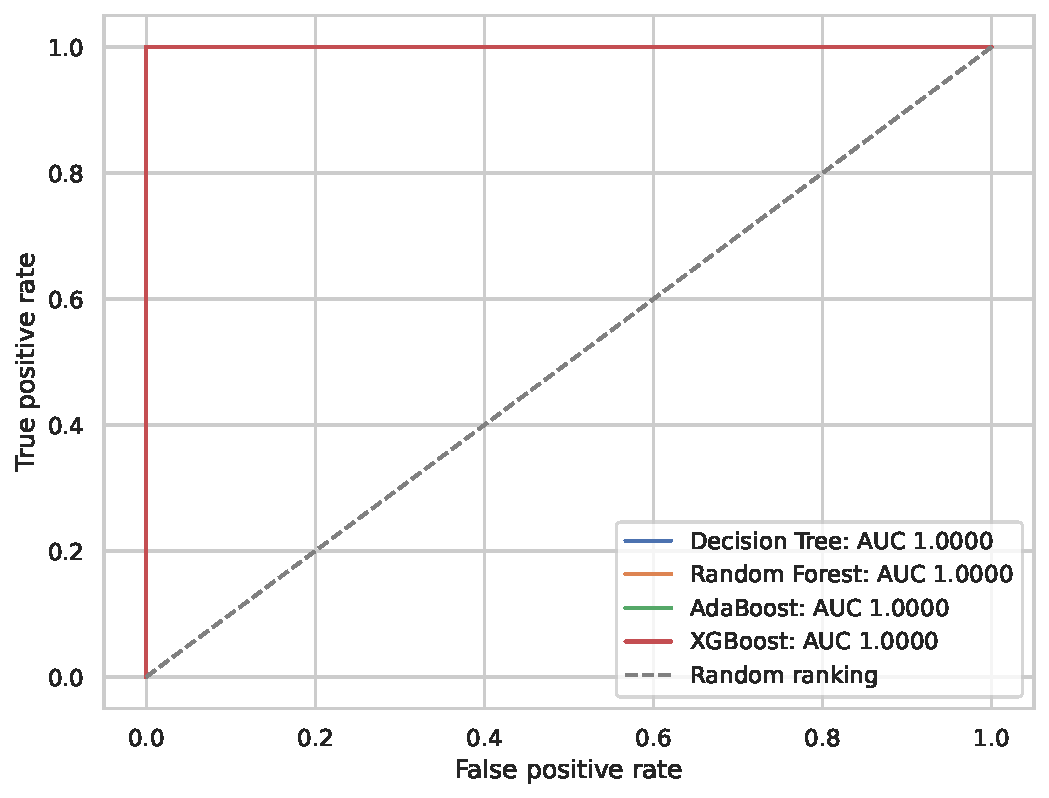
\includegraphics[width=.49\linewidth]{10_roc_curves.pdf}\hfill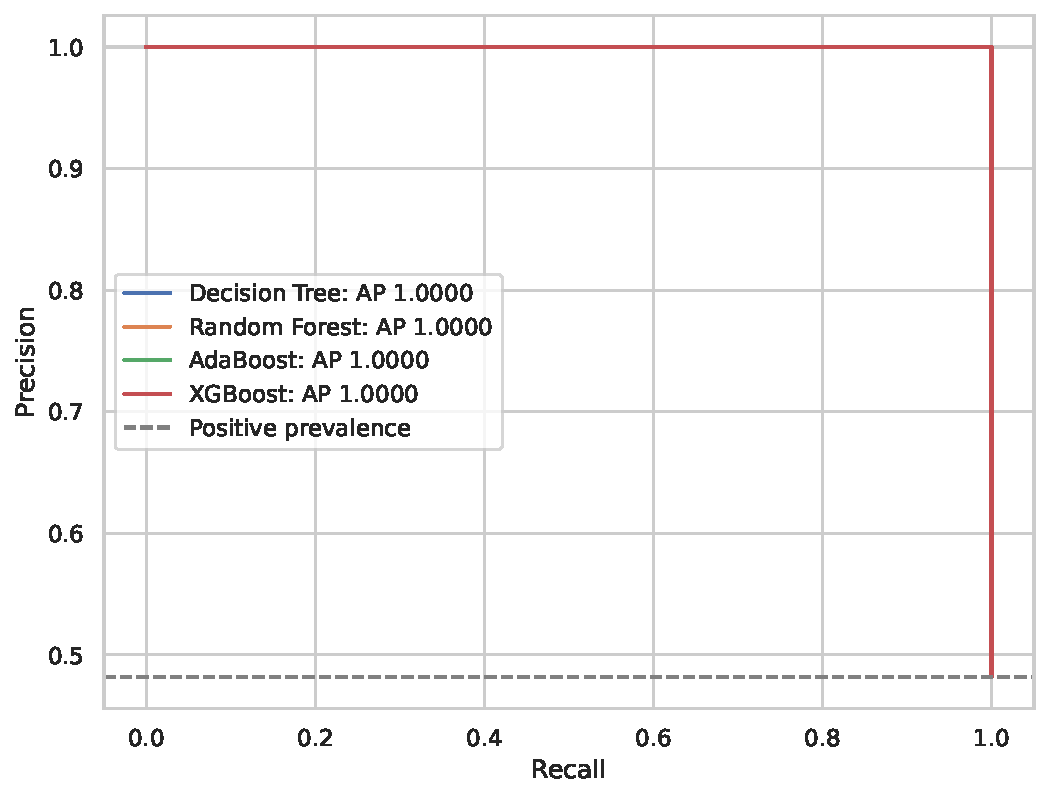
\includegraphics[width=.49\linewidth]{11_precision_recall_curves.pdf}
\caption{ROC and precision-recall curves overlap for the four fitted models. Overlap is an evaluation ceiling, not evidence of identical probabilities.}\end{figure}
ROC plots sensitivity against the false-positive rate while the threshold changes. AUC 1.0 means every positive score exceeds every negative score in this partition. Precision-recall shows the corresponding retrieval tradeoff; the horizontal reference is positive prevalence, 783/1,625 or 0.4818. Average precision summarizes precision at recall increments, rather than a separately computed trapezoidal PR area. AP 1.0 shows complete separation. Neither plot measures whether a score of 0.60 means a 60\% event rate. They cannot distinguish these models at this test-set ceiling.

\begin{table}[H]
\centering\small
\caption{Test-set probability quality. Smaller losses are better.}
\begin{adjustbox}{max width=\linewidth}\begin{tabular}{lrr}
\toprule
Model & Brier & Log loss \\
\midrule
Decision Tree & 0.000000 & 0.000000 \\
Random Forest & 0.000056 & 0.001376 \\
AdaBoost & 0.149355 & 0.487553 \\
XGBoost & 0.000020 & 0.001435 \\
\bottomrule
\end{tabular}\end{adjustbox}
\end{table}

\begin{figure}[H]\centering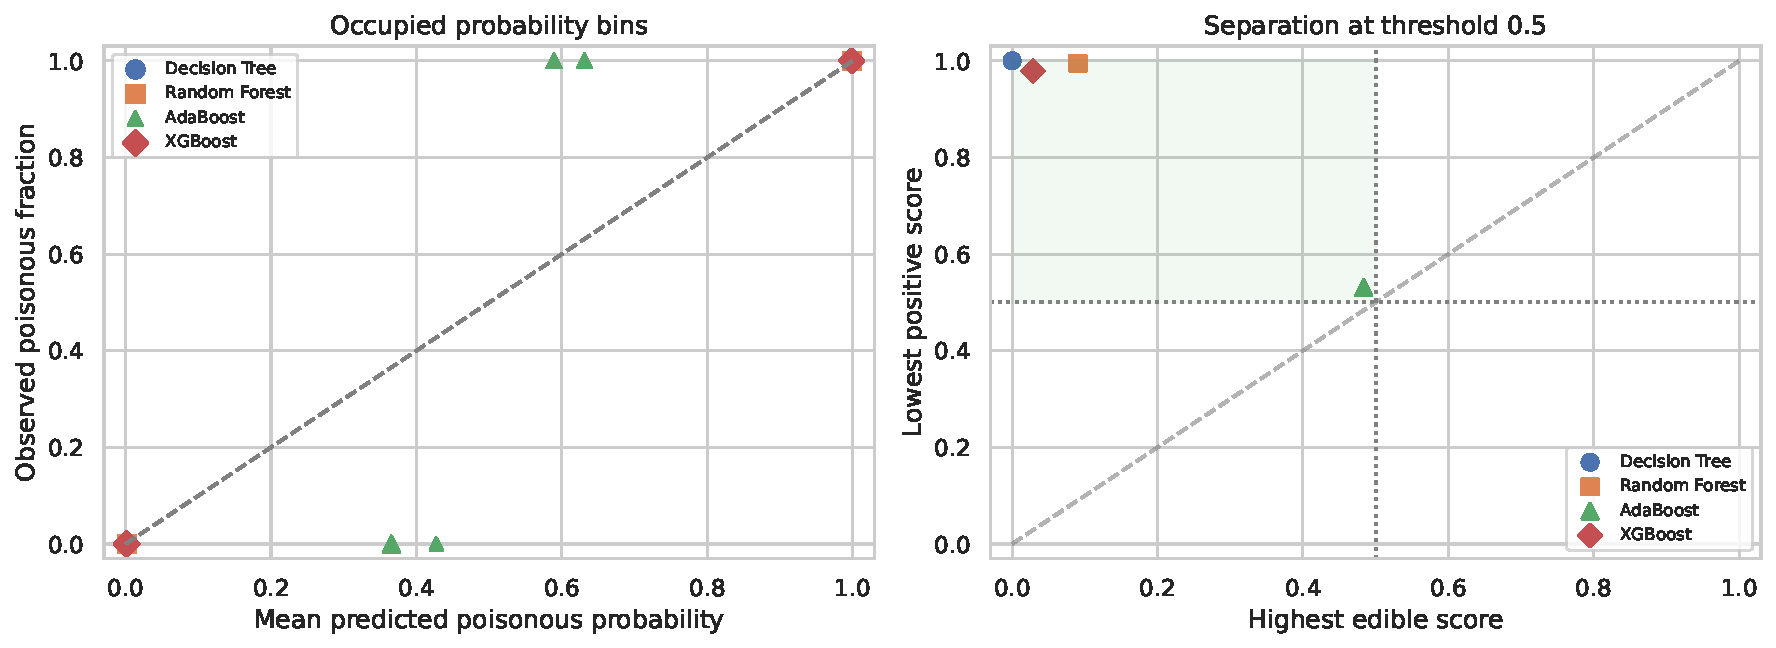
\includegraphics[width=\linewidth]{13_probability_quality.pdf}\caption{Observed frequencies in occupied probability bins, with marker area reflecting row support. The dashed diagonal is ideal agreement. On the right, the shaded upper-left region marks perfect classification at threshold 0.5: the highest edible score is below 0.5 and the lowest positive score is above it.}\end{figure}
The four models separate the classes, but their confidence differs. Pure Decision Tree leaves assign zero or one on this test set. AdaBoost places scores much closer to 0.5, which gives substantially worse probability losses despite identical correct labels. The gap between the highest edible score and lowest positive score explains why these moderate probabilities still produce perfect classification. Score ordering and score magnitude answer different questions. The occupied bins contain 842 edible and 783 positive rows for each of the other three models. AdaBoost spreads those classes across four bins with 646, 196, 397 and 386 rows. The plot shows occupied bins without joining them; no probability reliability is established in the empty intervals.
The notebook checks that the installed AdaBoost implementation transforms its normalized weighted voting margin through a logistic function to obtain the binary probability. A correct weighted-vote sign can therefore coexist with moderate confidence; the score is not an empirical class frequency from a pure leaf. Brier score is mean squared probability error; log loss penalizes assigning low probability to the observed class. Scikit-learn clips extreme probabilities at floating-point precision for log loss, so zero-or-one scores yield finite penalties. The six-decimal probability tables can round a very small loss to zero. These losses assess overall probability quality, including discrimination and reliability, rather than isolating calibration alone \cite{sklearn_calibration}. A Decision Tree can issue pure-leaf probabilities of zero and one here, but that behavior is not a guarantee of reliable probabilities under shift. No calibration model or new threshold is fitted on test labels.

\section{Why perfect row-split results are not the whole answer}
\begin{table}[H]
\centering\small
\caption{Exact predictor-profile coverage. Test size is 1,625 rows.}
\begin{adjustbox}{max width=\linewidth}\begin{tabular}{lrrrrr}
\toprule
Policy & Attributes & Train profiles & Test profiles & Seen test rows & Mixed profiles \\
\midrule
All original attributes & 22 & 6499 & 1625 & 0 & 0 \\
Seven-attribute prefix & 7 & 174 & 171 & 1625 & 0 \\
Selected Decision Tree & 5 & 47 & 46 & 1625 & 0 \\
\bottomrule
\end{tabular}\end{adjustbox}
\end{table}

The original 22-feature descriptions are unique, yet reduced representations collapse many rows into the same profile. The table measures exact combinations without using labels. Every test row has a selected Decision Tree profile already present in training. Training profiles are class-pure. The independently refitted row-CV models also export validation-profile coverage in every fitting fold. A training-only profile lookup therefore also achieves perfect test-set classification. This is not direct target leakage: the lookup uses training labels only. It shows that the partition tests familiar profiles and gives little evidence about unfamiliar combinations. The dependence also cautions against simple independent-row confidence bounds.

We address that gap with a stress test restricted to the training partition. The five traits selected on the full training set define 47 fixed groups. Five StratifiedGroupKFold splits hold these groups apart: no fixed grouping profile crosses a fold boundary. Each pipeline retains its chosen settings but refits its feature ranking inside the fitting fold. Consequently, its actual selected traits can differ from the five used for grouping. Distinct groups can then become identical model inputs; 981 validation rows per model have such familiar inputs. This is a test of holding the fixed groups apart, not a test in which every model input is unfamiliar. The grouping was chosen during development, and settings are not reselected inside each outer fold. The result is a conditional diagnostic, not an unbiased nested estimate of the whole selection procedure or evaluation across identified species \cite{sklearn_validation}.
\begin{table}[H]
\centering\small
\caption{Stress test with fixed five-trait groups held apart. Metrics pool five validation folds of training rows.}
\begin{adjustbox}{max width=\linewidth}\begin{tabular}{lrrrrrr}
\toprule
Model & Accuracy & Precision & Recall & F1 & FN & FP \\
\midrule
AdaBoost & 0.9648 & 0.9575 & 0.9700 & 0.9637 & 94 & 135 \\
Decision Tree & 0.9771 & 0.9822 & 0.9700 & 0.9761 & 94 & 55 \\
Profile lookup fallback & 0.5179 & 0.0000 & 0.0000 & 0.0000 & 3133 & 0 \\
Random Forest & 0.9771 & 0.9822 & 0.9700 & 0.9761 & 94 & 55 \\
XGBoost & 0.9802 & 0.9886 & 0.9700 & 0.9792 & 94 & 35 \\
\bottomrule
\end{tabular}\end{adjustbox}
\end{table}

\begin{figure}[H]\centering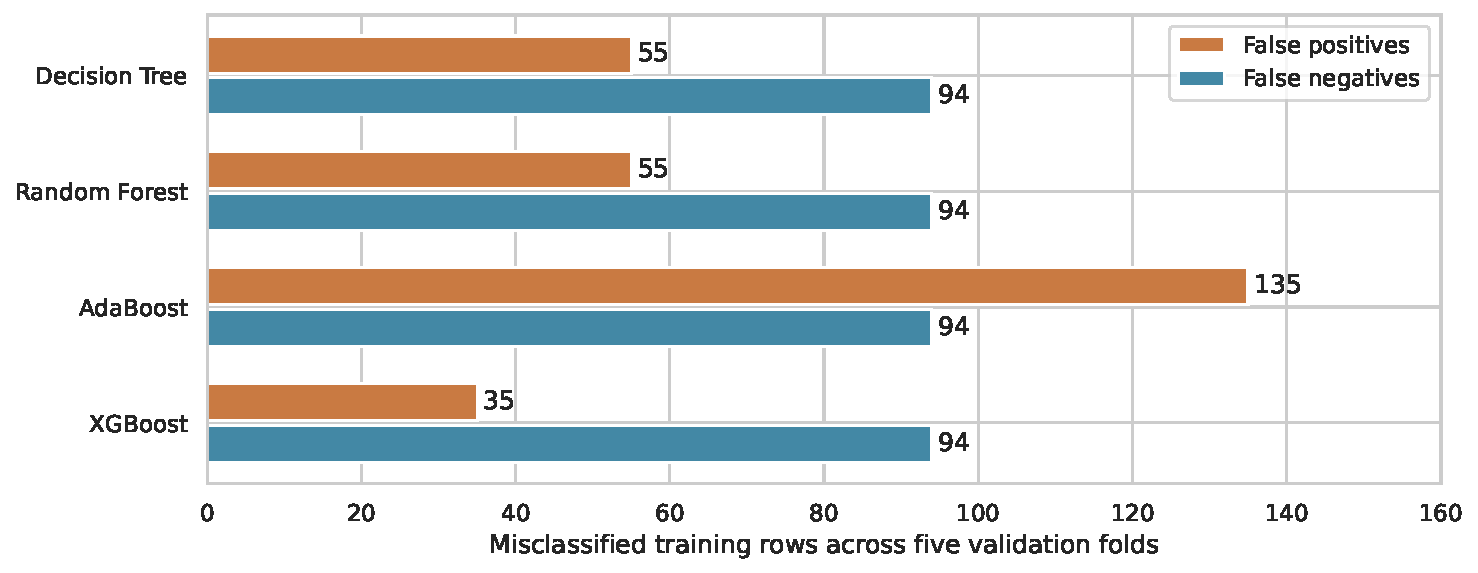
\includegraphics[width=.95\linewidth]{14_group_stress.pdf}\caption{Pooled error counts for the four fitted models with fixed five-trait groups held apart. All models miss the same 94 positive rows. XGBoost reduces false positives; some inputs remain familiar under fold-selected traits. The lookup baseline is retained in the preceding table.}\end{figure}
The perfect row-split ceiling disappears when the fixed groups are held apart. XGBoost has the highest pooled F1 (0.9792) in this specified stress test; the Decision Tree has F1 0.9761. The evaluation removes exact overlap under the fixed grouping definition, although it does not remove all overlap under the models' fold-selected traits. All four methods miss the same 94 positive odorless rows. Their recall is identical; the XGBoost gain comes from 20 fewer false positives than the Decision Tree, or 0.31 percentage points of accuracy across 6,499 rows. It does not improve recovery of these exceptions. The stability of this small advantage across other group partitions is not established. The largest erroneous Decision Tree profile has 56 validation rows: odor=none; spore-print-color=green; ring-type=pendant; stalk-surface-below-ring=smooth; gill-size=broad. It produces 56 false negatives and 0 false positives. The other missed positive groups are odorless, white-spored and narrow-gilled: 30 rows have an evanescent ring and scaly lower stalk; 8 have a pendant ring and smooth lower stalk. All 94 rows in these three groups are missed by every model. The failures concern entire combinations, not scattered errors within otherwise successful groups.
\begin{table}[H]
\centering\small
\caption{Equal-profile diagnostic averages. These are different weights from the pooled row metrics.}
\begin{adjustbox}{max width=\linewidth}\begin{tabular}{lrrrrr}
\toprule
Model & Profile accuracy & Positive recall & Edible specificity & Positive profiles & Edible profiles \\
\midrule
AdaBoost & 0.8298 & 0.8235 & 0.8333 & 17 & 30 \\
Decision Tree & 0.8723 & 0.8235 & 0.9000 & 17 & 30 \\
Profile lookup fallback & 0.6383 & 0.0000 & 1.0000 & 17 & 30 \\
Random Forest & 0.8723 & 0.8235 & 0.9000 & 17 & 30 \\
XGBoost & 0.8936 & 0.8235 & 0.9333 & 17 & 30 \\
\bottomrule
\end{tabular}\end{adjustbox}
\end{table}

Equal-profile averages reveal the cost of counting repeated common patterns many times. The 17 positive profiles include three exceptional odorless profiles, containing 56, 30 and 8 rows. All four methods miss those three profiles, so their equal-positive-profile recall is 0.8235, compared with pooled row recall 0.9700. These alternative weights are a diagnostic of coverage, not an asserted deployment distribution. A strong pooled score can coexist with failure on every profile in a small exceptional subgroup.
\begin{table}[H]
\centering\small
\caption{Probability quality with fixed five-trait groups held apart, pooled across five folds.}
\begin{adjustbox}{max width=\linewidth}\begin{tabular}{lrr}
\toprule
Model & Brier & Log loss \\
\midrule
AdaBoost & 0.160706 & 0.511020 \\
Decision Tree & 0.021321 & 0.739816 \\
Profile lookup fallback & 0.254681 & 0.702578 \\
Random Forest & 0.020999 & 0.403861 \\
XGBoost & 0.017483 & 0.170708 \\
\bottomrule
\end{tabular}\end{adjustbox}
\end{table}

With the fixed groups held apart, XGBoost has the smallest pooled Brier score and log loss. The Decision Tree can issue zero-or-one probabilities for pure leaves; wrong extreme scores incur especially large log penalties when a new profile follows the wrong rule. Thus pure training leaves can look ideal on familiar profiles and overconfident on unfamiliar ones. Of the Decision Tree's 149 stress errors, 133 have an exactly zero-or-one score. AdaBoost makes more label errors but has lower log loss than the Decision Tree here, because moderate wrong scores receive a smaller penalty. These are conditional pooled diagnostic losses; no probability calibration is fitted on these validation labels.
\begin{table}[H]
\centering\small
\caption{Stress-test errors with and without new category levels in selected attributes.}
\begin{adjustbox}{max width=\linewidth}\begin{tabular}{lrrrrr}
\toprule
Model & Rows & Seen profiles & New levels & Errors, new levels & Errors, seen levels \\
\midrule
AdaBoost & 6499 & 981 & 1276 & 56 & 173 \\
Decision Tree & 6499 & 981 & 1276 & 56 & 93 \\
Random Forest & 6499 & 981 & 1276 & 56 & 93 \\
XGBoost & 6499 & 981 & 1276 & 56 & 73 \\
\bottomrule
\end{tabular}\end{adjustbox}
\end{table}

All four models have 56 errors involving unseen category levels. These are the green-spore odorless profile: its positive rule cannot be learned when that category is absent from fitting data. The encoder can represent an unknown level computationally, but cannot infer its label from its name. The remaining two positive odorless profiles contain 38 rows whose individual levels are represented in fitting data. Their failure concerns a new conjunction, showing why familiar categories do not guarantee a familiar decision rule. As noted when defining the experiment, 981 validation rows per model have familiar inputs under the fold-selected traits. Table 15 separates this input overlap from unseen individual category levels; these are different forms of coverage. These are descriptive strata, not causal attributions. The latter errors expose difficulty with new combinations rather than simply a missing encoder category. The decoded error-profile file identifies the precise conjunctions and class support.
The profile lookup cannot use an exact match because all validation groups are unfamiliar, so its fallback provides a reference for predicting without an exact match under the grouping definition. The model comparison also reflects changed feature selection and some familiar inputs; it does not isolate interpolation alone. Each validation fold has different group sizes and class support. We pool predictions for the main comparison and retain fold metrics and counts rather than treating the average of unequal folds as the only answer. All validation row IDs, groups, predictions, probabilities and selected attributes are exported. This stronger diagnostic shows why a ceiling on the random row split must not end the analysis.

\section{Recommendation and assumptions}
For explaining the familiar test-set profiles, the Decision Tree is preferable: it matches the four models' classification scores with one readable rule system and far fewer fitted leaves. That recommendation is based on interpretability and measured complexity, not superior test-set F1. The stronger limitation is shared by all four methods: holding the fixed groups apart leads to failure on all 94 rows in the three positive odorless groups. In the grouped stress test, XGBoost has the best observed F1, Brier score and log loss. Its classification advantage comes entirely from fewer false positives. It does not solve the missed positive exceptions, and the small F1 advantage has not been shown to persist across other group partitions. AdaBoost's moderate scores should therefore be judged in the evaluation setting rather than dismissed solely for their losses on familiar profiles. Selection for another deployment objective would need an independently collected evaluation set, an explicit error-cost policy and a probability-quality objective.

We assume the UCI label definitions and category dictionary are authoritative; missing root is an unknown category; each supplied row is a valid dataset description; the positive label is the evaluation target; and the source remains the same version. We retain uncommon levels rather than merge them without domain support. The exact source fingerprint, package versions, seeds, row IDs and selected settings are exported. These assumptions support a reproducible dataset comparison, not real-world edibility advice.

The main unresolved scientific limits are absent species or specimen identifiers, hypothetical source descriptions, unknown missingness mechanism, and the previously evaluated test set. The group experiment probes one specified form of shift, with only a small number of distinct groups. It cannot certify all shifts. No report claim substitutes fitted associations for causal biology or converts observed perfect scores into safety guarantees.

\clearpage
\appendix
\section{Complete preprocessing evidence}
\begin{longtable}{lrr}
\caption{Known category counts and missing values in all records.} \\
\toprule
Attribute & Levels & Missing \\
\midrule
\endfirsthead
\caption[]{Known category counts and missing values in all records.} \\
\toprule
Attribute & Levels & Missing \\
\midrule
\endhead
\midrule
\multicolumn{3}{r}{Continued on next page} \\
\midrule
\endfoot
\bottomrule
\endlastfoot
cap-shape & 6 & 0 \\
cap-surface & 4 & 0 \\
cap-color & 10 & 0 \\
bruises & 2 & 0 \\
odor & 9 & 0 \\
gill-attachment & 2 & 0 \\
gill-spacing & 2 & 0 \\
gill-size & 2 & 0 \\
gill-color & 12 & 0 \\
stalk-shape & 2 & 0 \\
stalk-root & 4 & 2480 \\
stalk-surface-above-ring & 4 & 0 \\
stalk-surface-below-ring & 4 & 0 \\
stalk-color-above-ring & 9 & 0 \\
stalk-color-below-ring & 9 & 0 \\
veil-type & 1 & 0 \\
veil-color & 4 & 0 \\
ring-number & 3 & 0 \\
ring-type & 5 & 0 \\
spore-print-color & 9 & 0 \\
population & 6 & 0 \\
habitat & 7 & 0 \\
\end{longtable}

\begin{figure}[H]\centering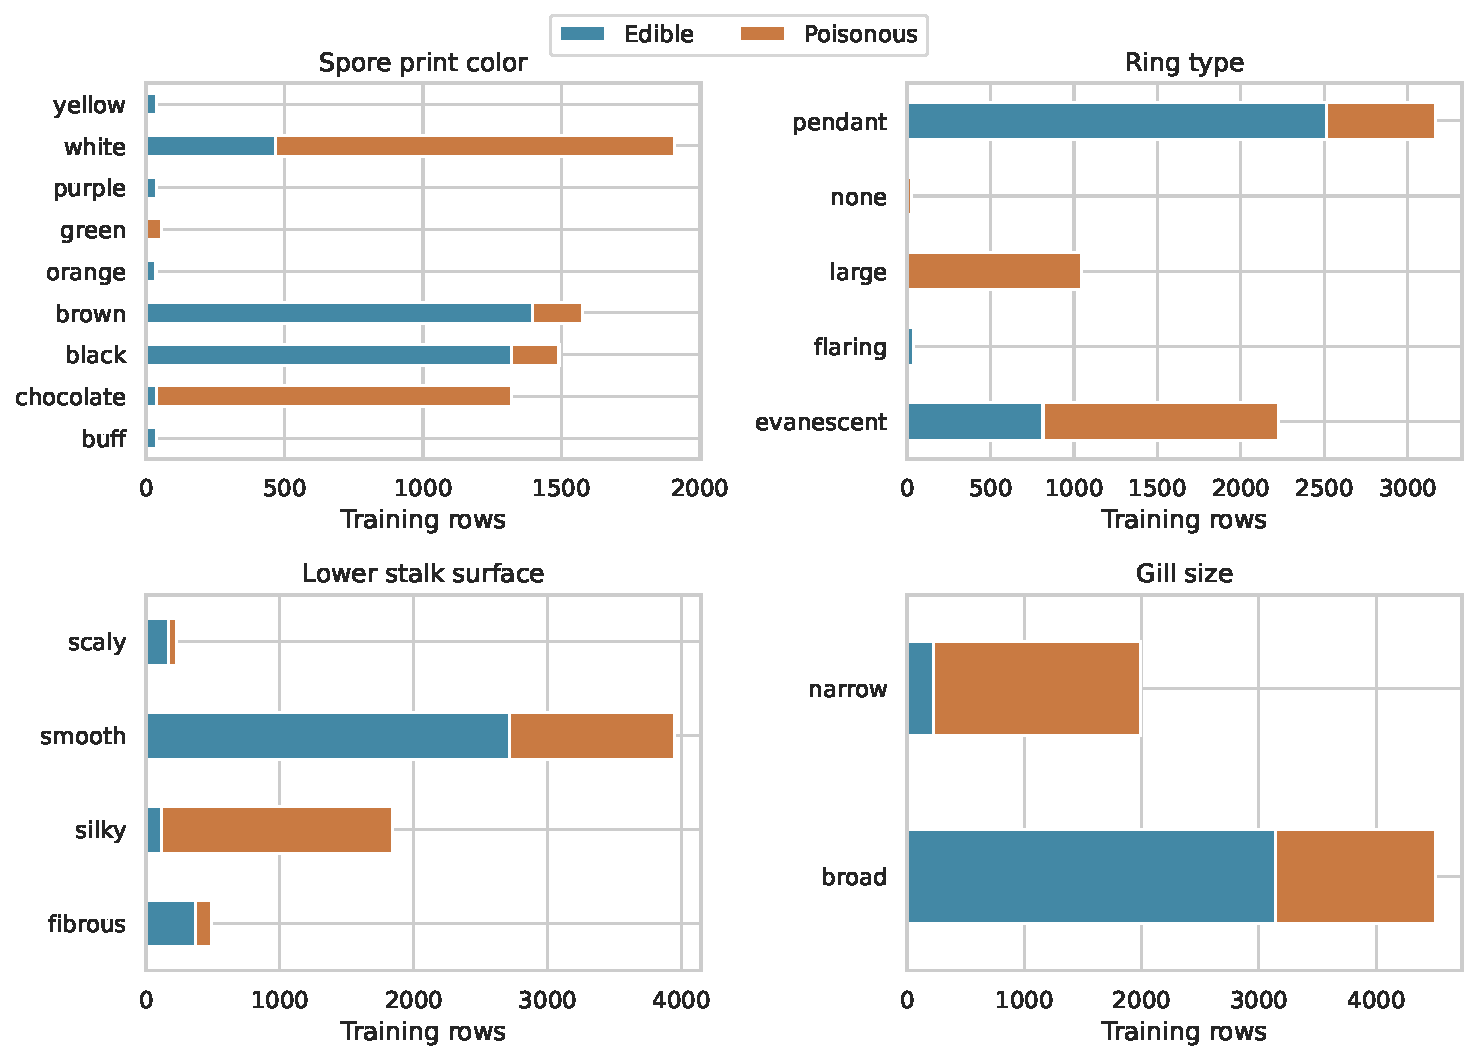
\includegraphics[width=\linewidth]{16_selected_trait_counts.pdf}\caption{Class-conditional counts for the other selected Decision Tree traits. The notebook exports distributions for all 22 original predictors.}\end{figure}
\begin{figure}[H]\centering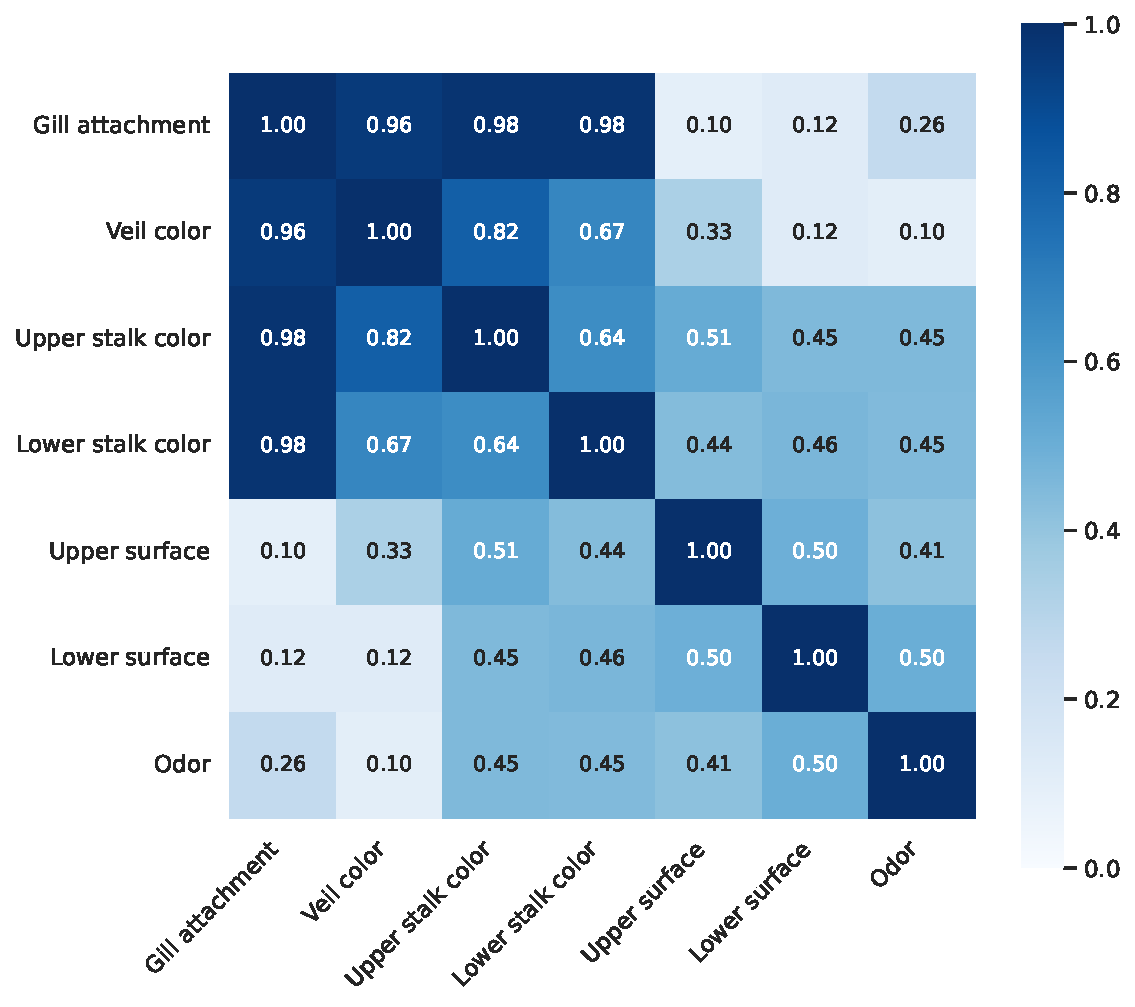
\includegraphics[width=\linewidth]{17_focused_associations.pdf}\caption{Focused training predictor associations. The full numerical matrix and 21-trait heatmap are supplied with the notebook. Values are Cramer's V.}\end{figure}
\section{Model grid values}
\begin{table}[H]
\centering\small
\caption{Model parameter values tested. Feature-policy choices are described separately.}
\begin{adjustbox}{max width=\linewidth}\begin{tabular}{lll}
\toprule
Model & Parameter & Values \\
\midrule
Decision Tree & max depth & 3.0, 6.0, None (unlimited) \\
Decision Tree & min samples leaf & 1, 5 \\
Random Forest & max depth & 6.0, None (unlimited) \\
Random Forest & max features & sqrt, 0.7 \\
Random Forest & min samples leaf & 1, 3 \\
Random Forest & n estimators & 100, 250 \\
AdaBoost & weak tree max depth & 1, 2 \\
AdaBoost & learning rate & 0.1, 0.5, 1.0 \\
AdaBoost & n estimators & 50, 150 \\
XGBoost & learning rate & 0.05, 0.2 \\
XGBoost & max depth & 2, 4 \\
XGBoost & n estimators & 100, 250 \\
\bottomrule
\end{tabular}\end{adjustbox}
\end{table}

\section{Ensemble tree examples}
\begin{figure}[H]\centering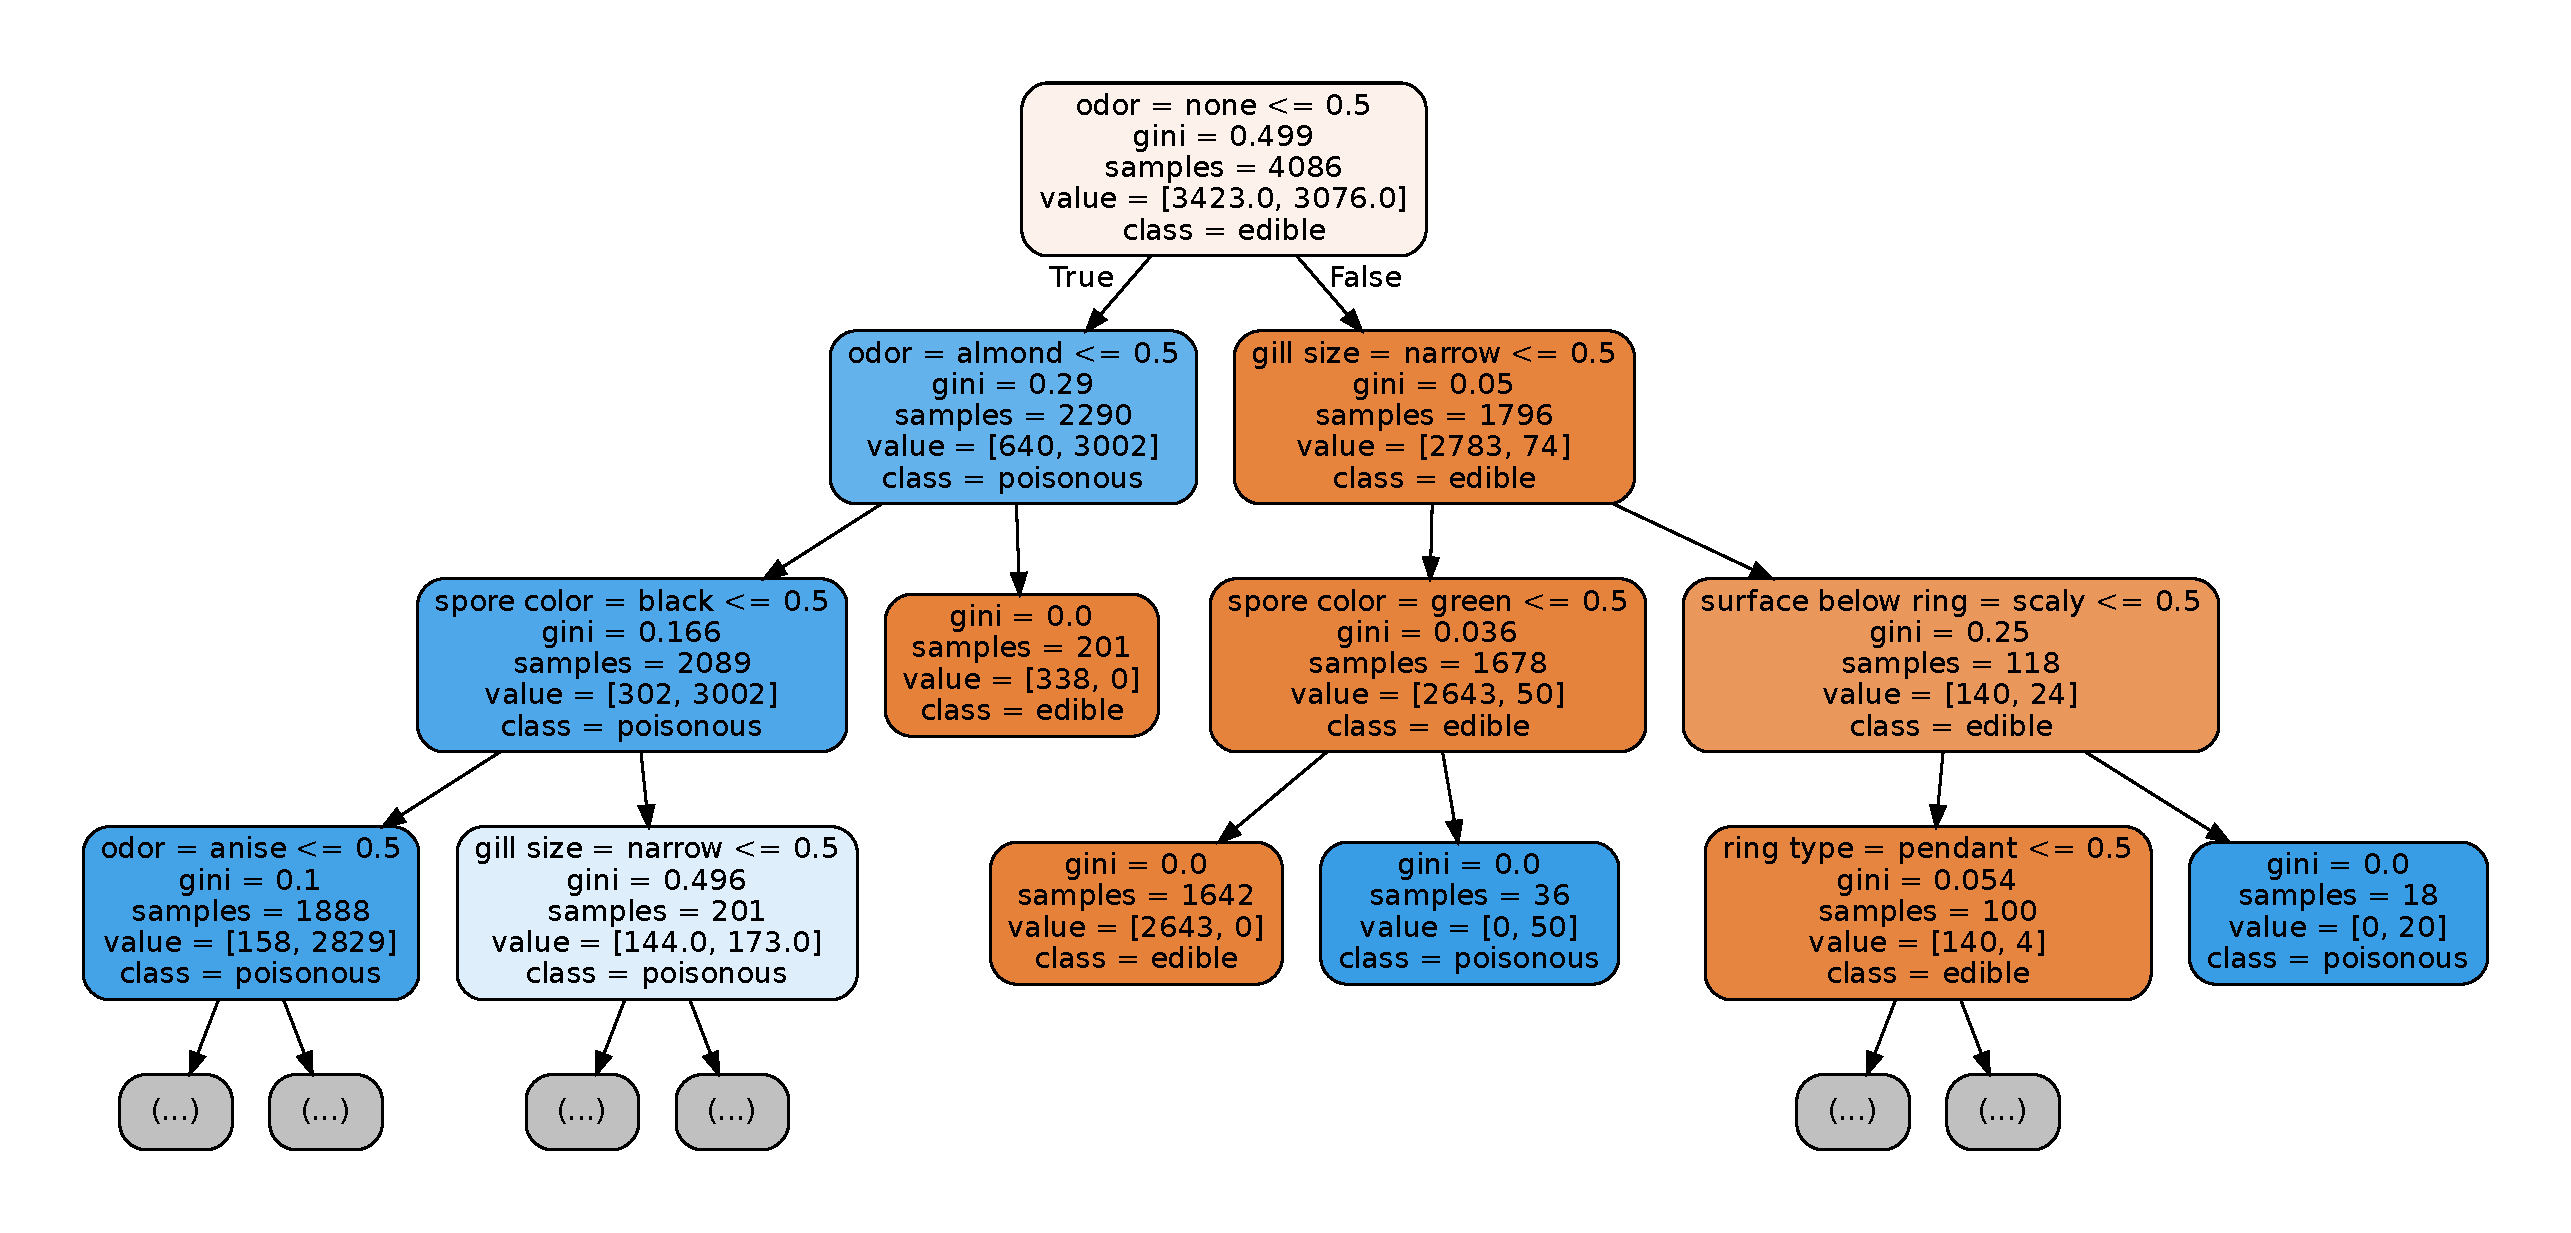
\includegraphics[width=\linewidth]{06_random_forest_tree.pdf}\caption{Root and first three split depths of the first Random Forest tree. Predictions aggregate the entire fitted forest.}\end{figure}
\begin{figure}[H]\centering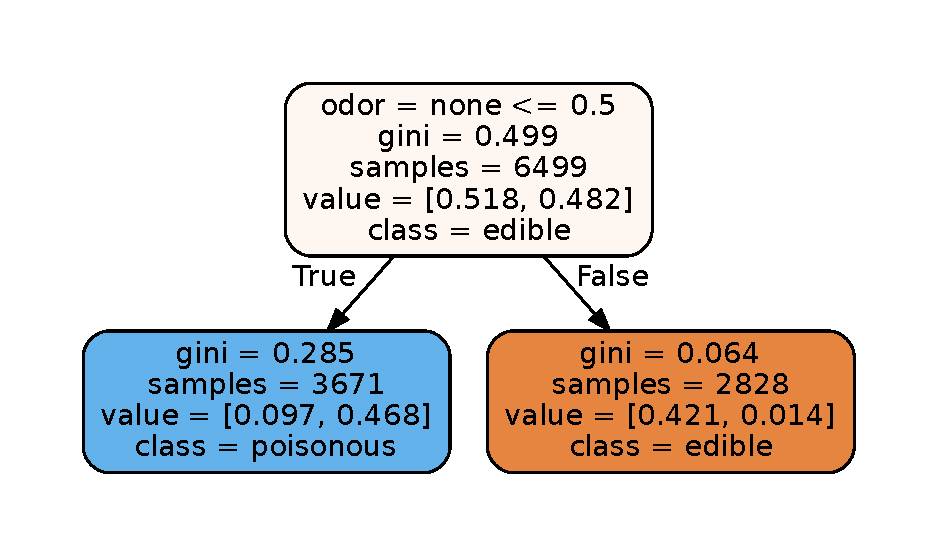
\includegraphics[width=.85\linewidth]{07_adaboost_tree.pdf}\caption{First AdaBoost weak tree. Values show weighted class mass as fractions of total fitting weight, not within-node probabilities or raw specimen counts. The non-odorless leaf contains about 0.097 edible and 0.468 positive mass; its positive fraction is therefore about 0.468/(0.097+0.468).}\end{figure}
\begin{figure}[H]\centering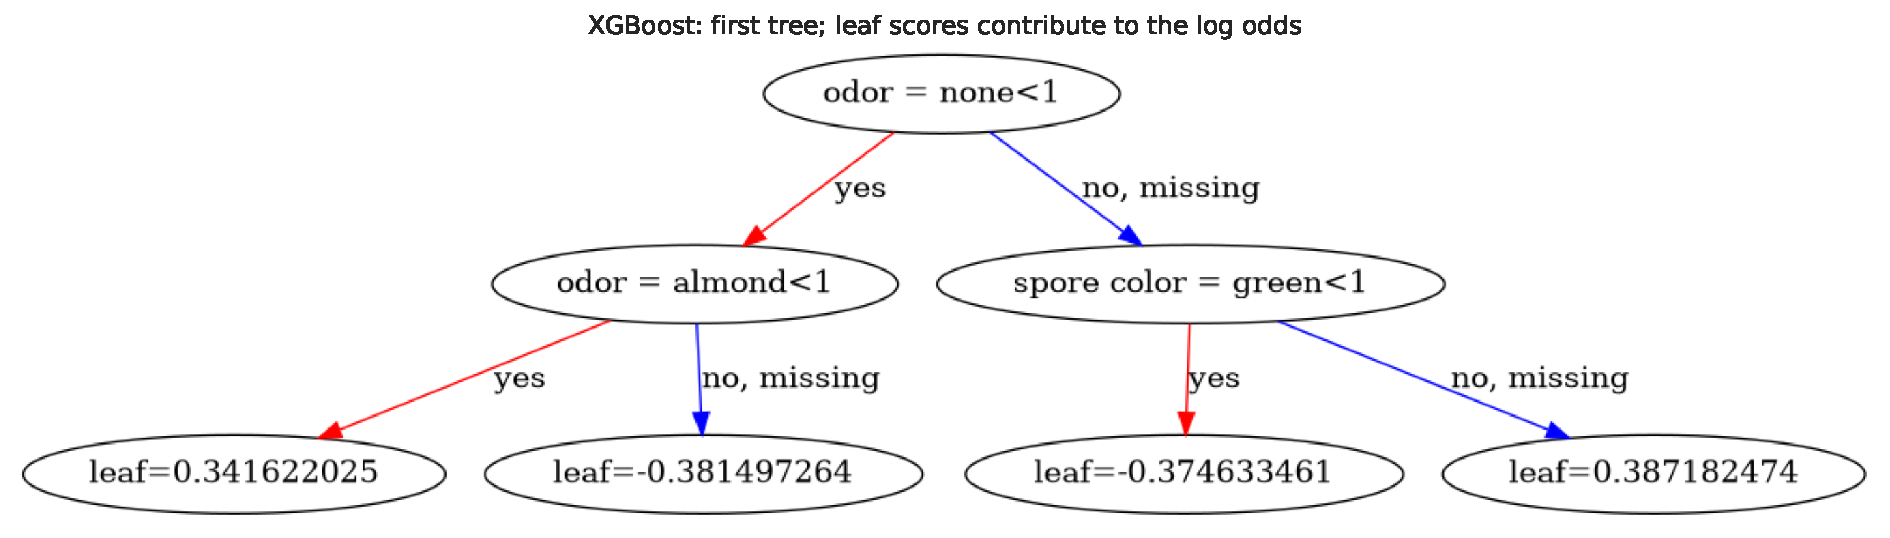
\includegraphics[width=\linewidth]{08_xgboost_tree.pdf}\caption{First XGBoost tree with decoded split names. Indicators are zero when a category is absent and one when present. The odorless, green-spored path reaches a positive leaf contribution of about 0.387, increasing the positive log odds. The non-odorless, almond path contributes about -0.381. Neither contribution alone determines the final probability; the initial score and all fitted trees are combined.}\end{figure}
\section{Reproducibility and assignment coverage}
The notebook fetches UCI dataset 73 through a public source, fits every preprocessing step inside training folds, searches all four model families, and regenerates figs/ and results/. The README gives environment, Graphviz and notebook execution instructions and LaTeX compilation commands. It also maps assignment requests to notebook sections and report evidence. Full grid outputs are supplied as CSV rather than hundreds of unreadable report rows. No code appears in this report and no raw dataset is included in the archive.
\begin{table}[H]
\centering\small
\caption{Support of the profile-held-apart validation folds.}
\begin{adjustbox}{max width=\linewidth}\begin{tabular}{rrrrrr}
\toprule
Fold & Fit rows & Rows & Fit groups & Validation groups & Validation poisonous \\
\midrule
1 & 4811 & 1688 & 37 & 10 & 1046 \\
2 & 5234 & 1265 & 43 & 4 & 526 \\
3 & 5295 & 1204 & 43 & 4 & 521 \\
4 & 5330 & 1169 & 33 & 14 & 516 \\
5 & 5326 & 1173 & 32 & 15 & 524 \\
\bottomrule
\end{tabular}\end{adjustbox}
\end{table}

\bibliographystyle{plainnat}
\bibliography{references}
\end{document}
